\documentclass[a4paper,12pt]{article}
\usepackage{natbib}
\usepackage{graphics}
%\usepackage{linguex}
\usepackage[utf8x]{inputenc}
\usepackage{ucs} %sami letters\renewcommand
%{\refdash}{}
\usepackage[T1]{fontenc}
\usepackage{multirow}
\usepackage{tabularx} %specified width
\begin{document}


\title{OAHPA -- pedagogical programs based on linguistic resources}

\author{Lene Antonsen, University of Tromsø}
\date{\today}
\maketitle
\pagenumbering{arabic}
 
\maketitle
\tableofcontents


\section{Introduction}
We wanted to use our linguistic resources for Sámi to make drills for students learning the language. We have developed five programs for North Sámi, which is the language with the best resources. In the next section I describe the linguistic resources we already had and the pedagogical idea behind the programs. In the third section I explain the different modules made for the pedagogical programs. The fourth section is about the design of each program. In the end I write a little about future plans.

We use the abbreviations for the sámi languages in accordance with the ISO 639-2 standard for language codes. The code is \textit{sme} for North Sámi. 

The work has been teamwork. Saara Huhmarniemi is the programmer, and together with her Trond Trosterud and I have planned the modules and designed the programs. Biret Ánne Bals Baal and I have worked with the lexicon and made question matrices. I have especially worked with the feedback and the dialogues, and written documentation and grammar. Kjellaug Isaksen has made drawings. The work is in the final stage now, and the programs will be made public in the beginning of February 2009. 

\section{Background}


\subsection{Existing linguistic resources}

The Giellatekno-project group at the University in Tromsø has made language resources for North Sámi based on morphological transducers because of that sámi languages have large paradigms for each lexeme. Each lexeme can have several tens of inflected forms; verbs and adjectives have more than 100 inflected forms. Some of the paradigm members have a very low text frequency, and there is not so much text electronically available. \citep{TT07}  

Using a morphological transducer one can analyse and generate every theoretically possible word form. Combining a dictionary with declension class info plus a morphological transducer will give a grammatical analyser, capable of analysing running text. Statistical approaches work best for languages with huge amounts of text electronically available, and a minimal amount of morphology. 
\citep{TT07}
\newpage
The existing language resources, which we have used in the pedagogical programs:
\begin{itemize}
\item a program for tokenization and processing (perl).
\item a morphological analyser/generator with finite state transducers, compiled with xfst. The system consists of a lexical transducer for morphology, lexc, and a phonological transducer, twolc. The lexicon contains 43.000 proper nouns, 31.000 common nouns, 14.000 verbs, 5.500 adjectives and 4.000 words of other word classes. One can compile two different variants of the analyser/generator -- \texttt{sme.fst/isme.fst} which is very tolerant, based on corpus, and \texttt{sme-norm.fst/isme-norm.fst} which is normative and a base for the North Sámi speller.  
\item an interface to the morphological analyser/generator, lookup. 
\item a morphological disambiguator based on constant grammar with manually written rule sets (vislcg3). 
\item syntactic analyser which adds grammatical function and dependency (vislcg3). The dependency file is not finished yet.
\item number word generator, made with finite state transducers.
\end{itemize}

The Xerox tools are documented in \citep{BeesleyKarttunen}. vislcg3 is a new generation version of the open source vislcg, and documented .....

Text analysator, word generator, paradigm generator and number word generator is accessible on the Inernet: \textit{http://giellatekno.uit.no}

\subsection{The pedagogical idea}
We wanted to utilize our analysator to develop pedagogical programs for Sámi instruction. The idea was that they could be used as a tool for students training linguistic skills. 

With the analysator we had the possibility to make an intelligent language tutoring system with sophisticated error analysis where student tasks can go beyond multiple-choice questions or the string-matching-algorithms. Usually the cost of developing a such system is to big, but we had already the analysator.

We difined that important for the pedigogical programs was that:

\begin{itemize}
\item they should be very flexible: Teacher or student can choose exactly what they want to train, and adapt them to each student's linguistic level 
\item one should be able to restrict the vocabulary to particular schoolbooks so it is easy to integrate the tools to the instruction
\item the student should get immediately feedback about errors
\item the student should easily get translation and grammar help
\item the student and the teacher should be able to work with topics 
\item the programs should be accessable free for everybody on server on Internet, without installing new programs in the computer
\end{itemize}

Sámi is a language with complex morphology, and it demands a lot of practising before the student reaches necessary skills. But Sámi is a minority language and it is a common situation that the person learning Sámi, does not get chance to practise the language enough in a natural way. Because of that can programs accessable at Internet be a useful supplement to the instruction at school and university. We wanted also to make a dialogue program about everyday topics. The goal is to exercise verb inflection, choosing the correct case and learn more words. 

In North Sámi there are to main dialects, and it is an advantage to be able to choose dialect. Especially when training morphology, it is an advantage if the presented forms, are the same as one has learnt in the instruction, or have heard in the language society. But at the same time, the program should accept any correct orthographic word form from the student.

We got financial support to the work from the University of Tromsø, and the Sámi Parliament in Norway.

The main lexicon is used for analysing the student’s input, but we want a pedagogical lexicon for more information about the lemmas, and as a base for the quiz and grammar tasks. The lexicon should be relevant according to the education in Sámi in schools and the university. We want that the student can choose main dialect for the output-language of the programs. We need sentence generator for the tasks and a system for feedback based on the student’s input. We need also a system for the dialogue. Because North Sámi is used in three countries, we want that the student can choose the metalanguage. Even if we now are working only with North Sámi, we want the possibility for making the programs in other sámi languages as well.

\section{Modules}

\subsection{Pedagogical lexicon}

The main lexicon consists of the Sámi words, information about the consonant gradation and continuation class, as we see in Figure \ref{nounsmelex}.\\


\begin{figure}[htbp]
\begin{center}
\scalebox{.7}[.7]{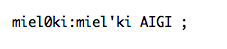
\includegraphics{img/noun-sme-lex.png}}\\
\caption{Example of entry in the main lexicon, noun-sme-lex.txt. AIGI is the continuation class.}
\label{nounsmelex}
\end{center}
\end{figure}

We wanted some more information in the lexicon. Therefore we made a special pedagogical lexicon in xml-format. I collected the lemmas, which were used in the schoolbooks and added Norwegian translation, information about semantic set, dialect and information about inflection. I also added information about source - which schoolbooks the lemma is used in. Read more about semantic sets in \ref{set}. The lexicon consists of 1538 nouns, 500 verbs and 194 adjectives. There is also a small lexicon for pronouns and numbers. In Figure \ref{nounlex} is an example of an entry in the nounlexicon. \\


\begin{figure}[htbp]
\begin{center}
\scalebox{.6}[.6]{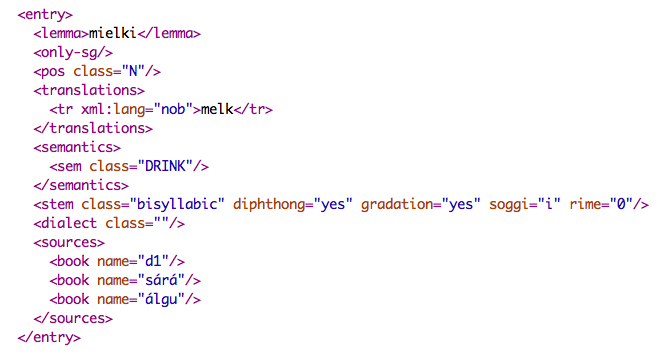
\includegraphics{img/nounlexicon.png}}\\
\caption{Example of entry in the pedagogical lexicon, nouns.xml}
\label{nounlex}
\end{center}
\end{figure}

Soma lemmas are homonomies in the base form. Because of different meanings they belong to different semantic sets. When the student wants the translation of the lemma, it should be the translations which belongs to the particular semantic set, e.g. \textit{girdi} can be both "plane" (VEHICLE) and "pilot" (PROFESSION). Other homonomies have different inflection, and it is critical to choose the correct lemma when we are generating word forms from it, e.g. \textit{bassi} Sg -- \textit{basit} Pl (= holy day) and \textit{bassi} Sg -- \textit{bassit} Pl (= washer). We have solved the problem by giving id to the critical entries, e.g. \texttt{id="girdi\_vehicle"} vs. 
\texttt{id="girdi\_profession"} and \texttt{id="bassi\_time"} vs. \textit{id="bassi\_actor"}.

%It works well as long as working with semantic classes, but if the user chooses "all" or a book, then he will not understand why the program doesn't accept his suggestions, e.g. girdi.

\subsection{System for dialectical variation}\label{dialect}
Saara - generation

We needed a strict generator. That means that the generator will generate only one word form for every grammatical word. The analysor is tolerant, but we have the opportunity of compiling two different analysators. We use \texttt{sme-norm.fst} for analysing the input and \texttt{isme-strict.fst} for the generator. isme-strict.fst generates only one word form for every grammatical word.

Because of dialectical variation, we made two versions of \texttt{isme-strict.fst}. We marked relevant lines in our source code like this:
\begin {itemize}
\item NG (not generate for any of the dialects)
\item NOT-KJ (not generate for KJ-dialect) 
\item NOT-GG (not generate for GG-dialect)  
\end {itemize}

We see an example in Figure \ref{smelex}. We also marked entries in the pedagogical lexicon-files with NOT-KJ and NOT-GG. This system can easily be expanded with more dialects.


\begin{figure}[htbp]
\begin{center}
\scalebox{.7}[.7]{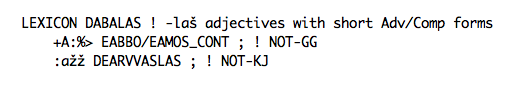
\includegraphics{img/smelex.png}}\\
\caption{In the makefile there are options to generate dialectical variants of word forms. From \texttt{sme-lex.txt}.}
\label{smelex}
\end{center}
\end{figure}


\subsection{System for feedback about morphology}

The information in the lexicon about inflection is there only to give a good feedback to the student. If s/he doesn't inflect the lemma correctly, s/he can choose to get hints about the inflection, and try once more, instead of getting the correct answer straight away. 

We make it in two steps. The first step is to define what kind of message should be given, based upon the combination of morphological features in the lexicon, and the inflection. In Figure \ref{feedbacknouns} is vowel changing in illative Sg defined for bisyllabic nouns which ends with the vowel "i":


\begin{figure}[htbp]
\begin{center}
\scalebox{.7}[.7]{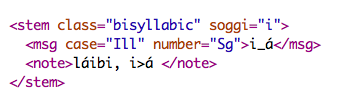
\includegraphics{img/feedback_nouns.png}}\\
\caption{The features in the lexicon are used to give message tags. Here the message tag is "i\_á". From feedback\_nouns.xml}
\label{feedbacknouns}
\end{center}
\end{figure}

This information is of course in the main lexicon also, but it is divided in two different automatons, lexc with the continuation lexicons and twolc for the consonant gradation, diphthong simplification and so on. If we are going to expand the pedagogical lexicon a lot, then it would be an advantage to generate the information directly from the main lexicon. 

The message tag is used to generate the feedback to the user. The message can be easily be translated into any language -- in Figure \ref{mess} it is in Norwegian.

\begin{figure}[htbp]
\begin{center}
\scalebox{.7}[.7]{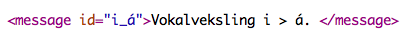
\includegraphics{img/messages.png}}\\
\caption{Feedback to the user is generated from the message tags. Here for the message tag "i\_á". From messages.xml.}
\label{mess}
\end{center}
\end{figure}

There are dialectical varieties in the orthography for some inflected forms, as explained under \ref{dialect}. And because of that, we have made two sets of feedback files, one for each dialect. But all the messages are in the same file, \texttt{messages.xml}.

In the example in the images above, the correct illative Sg word form of \textit{mielki} is \textit{mielkái}. As we see in Figure \ref{nounlex}, this lemma has the feature \texttt{only-sg}, which means that we generate the lemma only in singular, even if it according to the main lexicon, also can be used in plural. This information is for pedagogical reasons; it is not so natural to do use the plural form for a student on a lower level.

If our main lexicon had been in xml-format, then we could have put all this information there. It would be a better solution to maintain only one lexicon, instead of two.

\subsection{Sentence generator}\label{set}
To easily offer variation to the user, we use a sentence generator, instead of tailoring every question. The generator consists of question and answer matrices with variables representing sets of lemmas in the lexicon, as shown in Figure \ref{questionv}.

\begin{figure}[htbp]
\begin{center}
\scalebox{.7}[.7]{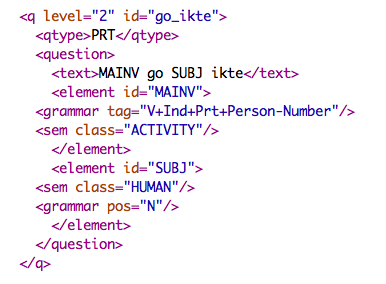
\includegraphics{img/question_vasta.png}}\\
\caption{Questions are generated. From questions\_vasta.xml.}
\label{questionv}
\end{center}
\end{figure}

The semantic sets are used both for the word quiz (Leksa) and the questions in Morfa-C and Vasta. There are ordinary sets and supersets, and one can choose which one suits best for the question, e.g. the big superset HUMAN with all lemmas for human beings, or a smaller subset, like PROFESSION. In Figure \ref{semset} is a definition of a superset. 

\begin{figure}[htbp]
\begin{center}
\scalebox{.7}[.7]{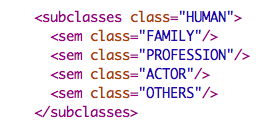
\includegraphics{img/semantic_set.png}}\\
\caption{Some of the semantic sets are supersets, consisting of subsets. From semantic\_sets.xml.}
\label{semset}
\end{center}
\end{figure}

We decide grammar for the variable. In this question the MAINV is in past tense because of the dividing into levels. In level 1 the student only get present tense. The tag, \texttt{Person-Number}, take care of the agreement with the SUBJ, and also for the required person and number in the answer. (Saara).

We chose not to accept inclusive pronouns, because we wanted the student to exercise all persons and numbers. Using inclusive pronouns, s/he could answer with the same verbform as in the question. The question Person-Number (QPN) Sg1 requires answer Person-Number (APN) Sg2, and so on:\\


\begin{tabular}[t]{rlrlrlrlrlr}
&QPN &APN &QPN &APN &QPN &APN \\
\hline
&Sg1 &Sg2 &Du1 &Du2 &Pl1 &Pl2 \\
&Sg2 &Sg1 &Du2 &Du1 &Pl2 &Pl1 \\
&Sg3 &Sg3 &Du3 &Du3 &Pl3 &Pl3 \\
\end{tabular}

\subsection{Analysator for student's input}\label{sentencefeedback}
We have chosen not to use multiple choice, but let the student formulate his own answers. That means that we have to analyze the answer. To a certain question one can give many kinds of acceptable answers. In Sámi you can change word order, and also add many kinds of particles.\\

\textit{Maid don lohket ikte?} (What did you read yesterday?)
\begin{itemize}
\item \textit{Mun han lohken ollu áviissaid.} (I PART read many newspapers.)
\item \textit{Ikte mun gal lohken buori girjji.} (Yesterday I PART read a good book.)
\item \textit{In lohkan maidege.} (I did not read anything.)
\item \textit{Ikte in lohkan.} (Yesterday I did not read.)
\end{itemize}


But the answer can contain grammar errors:
\begin{itemize}
\item \textit{Mun lohket ollu áviissaid.} \\ $\rightarrow$ Remember agreement between subject and verbal.  
\item \textit{Mun lohken ollu áviissat.} \\ $\rightarrow$ There should be an accusative in your answer. 
\item \textit{Don lohket ollu áviissaid.} \\ $\rightarrow$ Are you sure that you answer with the correct person?  
\end{itemize}

We use Vislcg3 for analysing the student's input. But first both the question and the answer are analysed with lookup to \texttt{sme.fst} and then the result is adjusted to cg3-format with a script. We use a file \texttt{ped-sme.cg3} which consists of only the first part of the morphological disambiguating in the \textit{sme-dis.rle} file, because there will probably be grammar and orthographic errors in the input. Instead of mapping syntactic tags to the words, we map tags for giving feedback to the student, or for navigating to the correct next question of in the dialogue, due to the student's answer.

Here I want a figure - with help of TTs program:\\
Q-A --- lookup to sme-norm.fst --- script lookup2cg --- vislcg3: ped-sme.cg3 --- generate message or navigation
Figure: fafdfsa\\

Q-A is the question and the student's answer. The script \texttt{lookup2cg} transforms the output of the lookup to correct format for vislcg3. How to generate messages is explained below.

The question mark in the Q-A is changed with a special symbol ("qst" QDL), because we do not want the question mark to be a delimiter in the analyse, but still we want the opportunity to make rules according to what is in the question (on the left side of the QDL).


\subsubsection{Tutorial feedback}
Tutorial feedback is feedback about grammar errors (prefix is \&grm), or that the student does not use the verb or noun, which s/he is supposed to do (prefix is \&sem). In Figure \ref{cg3} we see a rule for giving a message if the student has not used accusative, when the question requires one. 

\begin{figure}[htbp]
\begin{center}
\scalebox{.6}[.6]{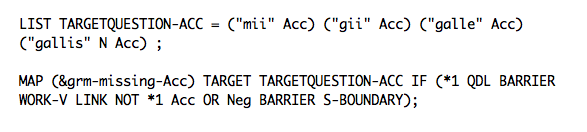
\includegraphics{img/pedcg3.png}}
\caption{Due to the question, we expect an accusative in the answer, if the question is not asking about infinitive, e.g. "What do you do?" (WORK-V). From sme-ped.cg3}
\label{cg3}
\end{center}
\end{figure}

\begin{figure}[htbp]
\begin{center}
\scalebox{.6}[.6]{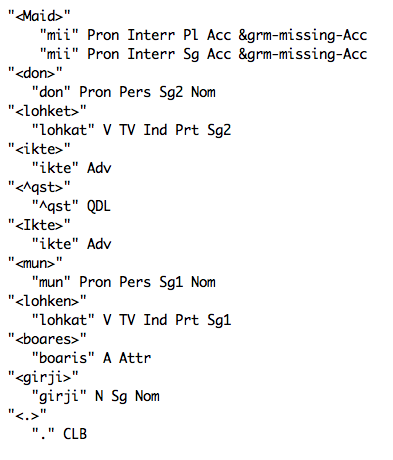
\includegraphics{img/maid_lohket_ikte.png}}
\caption{The tag is added to the interrogate. (What did you read yesterday qst Yesterday I read an old book (Nom instead of Acc))}
\label{maidlohket}
\end{center}
\end{figure}



\begin{figure}[htbp]
\begin{center}
\scalebox{.65}[.65]{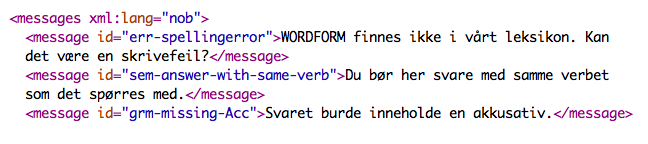
\includegraphics{img/messages_vasta.png}}
\caption{The tutorial message is generated from messages\_vasta.xml, and can be given in any language.}
\label{messv}
\end{center}
\end{figure}

%spelling errors (unknown input strings)
%grammatical errors (known and erroneous input strings)

The biggest problem is the student's spelling errors. It is not a problem if the spelling error makes a not-existing word form. Then the message to the student is  "The word form is not in our lexicon, can it be a spelling error?". The spelling error can make another word form of the same lemma. For that we make rules based on context. The real problem is when the spelling error makes an unintended lemma. Here are some examples and how we try to handle them:\\

\begin{itemize}

\item \textbf{Gluing locative suffix directly to the stem} \\
In our pedlexicon are 1512 nouns. By adding the suffix -s directly to the stem without consonant gradation, the result is 57 \% correct lemma but unintended word form (possessive suffix in Sg3 -- e.g. \textit{viessus} instead of \textit{viesus}). Only 0,5 \% of the word forms are unintended lemmas, e.g. adverbs \textit{eanas  (eatnamis)} or verbs, e.g \textit{čogus (čohkumis)}.

The possessive suffices are quite seldom used by students at lower levels, so if it does not fit to the context, one can assume that s/he has meant locative, and give feedback according to that. 

\item \textbf{Gluing illative suffix directly to the stem}\\
By adding the suffix -i or -ii directly to the stem without consonant gradation, vocal changing or diphthong simplification, we get 2,3 \% unintended lemmas, mostly verbs in past tense Sg3, e.g. \textit{báddii (báddái)}. Generally one can consider to identify problematic word pairs and make rules for them to give feedback and ask the student if s/he meant the other one, especially when we are not expecting one more finite verb.

\item \textbf{Incorrect negative verb form}\\
When the verb in the question is in Sg2, a common error is that the student use the Sg2 form of the verb after the negative verb, instead of the correct ConNeg form, e.g. \textit{Logat go áviissa? In logat (loga) áviissa.} The correct form is in the parentheses. The problem is that this form is a ConNeg form of another verb, \textit{logadit}, and the normal feedback will be: "You should answer with the same verb as in the question." The student will not understand this, because s/he thinks that it is the same verb. The solution was to generate all these forms of the verbs in the questions, make a set of them, and make a rule for in the right context, give the feedback: "The negative form is not correct.". 
\end{itemize}


\subsubsection{Navigating in the dialogue}
We use the same system to navigate inside the dialogue. The input is tagged with information about if it is affirmative, negative, and with target-tag, so we can pick up e.g. name, and use it in the next question or utterance. 

Some dialogues are branched according to how the student answer e.g. about having a car, or like in the answer from the student about the age, gives a tag (Figure \ref{age}), which is used to navigate to different branches of the dialogue, see Figure \ref{branch}.


\begin{figure}[htbp]
\begin{center}
\scalebox{.7}[.7]{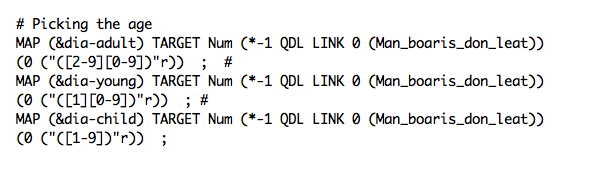
\includegraphics{img/picking_age.png}}\\
\caption{Rules for giving age-tag to the input. Special rule for the question named Man\_boaris\_don\_leat. From sme-ped.cg3.}
\label{age}
\end{center}
\end{figure}


\begin{figure}[htbp]
\begin{center}
\scalebox{.7}[.7]{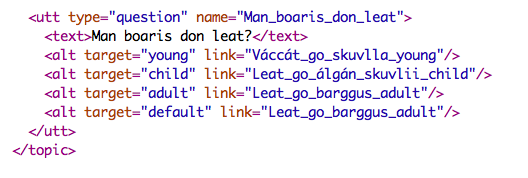
\includegraphics{img/Man_boaris.png}}\\
\caption{Example of how to navigate to the next question or branch, with help of the tag.  The question is "How old are you?" and the branches are adapted to the age of the student.}
\label{branch}
\end{center}
\end{figure}

As we see in the Figures \ref{maidlohket} and \ref{manboaris}, the questions in the dialogues are not generated, but tailored. Every question has it's own unique name, so we can link to it, and it is also possible to make a rule for a special question, like here.  

\section{The design of the pedagogical programs}
To all programs we have tried to make a not so technical look, so we have added drawings to the programs. The user can choose between two main dialects, and between four metalanguages (Norwegian, North Sámi, Finnish and English), but now in the beginning is only Norwegian and North Sámi fully supported. The biggest task is to translate the lexicon and grammar into the other languages.  

In most programs the student get a score after doing one task. We have a file with encouraging comments connected to the size of score, where from the comment is chosen randomly.

\subsection{Numra -- numeral exercise}
The Numra program consists of the numeral automat TT . This automat has been available for users on the Giellatekno web page. We have extended is also handles ordinals in the same way.  

The student can choose to work from arabic to word, and from word to arabic. S/he can also decide the range of numerals: 0-10, 0-20, 0-100 and 0-1000. Numra present five tasks at a time. The student can try so many times s/he wants, and the answers are marked with symbols for correct or incorrect. The student can ask for the correct answers, and then s/he gets a score and a comment connected to the score.

The automat is easy to make, so we have made it in many sámi languages, also so the students can compare the languages. We have Numra for North, Lule, South, Inari and Kildin Sámi.\\ 


\begin{figure}[htbp]
\begin{center}
\scalebox{.7}[.7]{
\includegraphics{img/numra.png}}\\
\caption{http://victorio.uit.no/oahpa/numra/.}
\label{numra}
\end{center}
\end{figure}

\subsection{Leksa -- word quiz}
It can be difference between the word's translations in a dictionary, and the word a student writes in a quiz. It is important not to give "error" to the student if s/he has written an acceptable translation of the word in the quiz, even if it is not the dictionary translation. It can be the same word in a different orthography, a synonym, or another meanings of the Sámi word. Therefore we have added more synonyms and possible translations to the dictionary.

"Leksa" works both from Sámi to Norwegian, and from Norwegian to Sámi. Therefore we have also made inverse versions of the lexicons. (Saara). In the original lexicon we have one-to-many entries, and we have uniqed the Norwegian entries in the inverse version, and there we also get there a one-to-many situation. Interesting to is that the nob-sme-lexicons are smaller than the sme-nob-lexicons: nouns, adjectives and verbs: 2232 entries in sme-nob vs. 1897 entries in nob-sme.\\ 

We have divided all the entries in the pedagogical lexicon into semantic sets, and they are put together in 17 supersets, e.g. nature, food/drink, clothing. The supersets consist of nouns, verbs and adjectives. The student can choose either to work with words from a schoolbook, or with a superset. 
\vspace{0.5cm}

\begin{figure}[htbp]
\begin{center}
\scalebox{.6}[.6]{
\includegraphics{img/leksa.png}}\\
\caption{http://victorio.uit.no/oahpa/leksa/}
\label{leksa}
\end{center}
\end{figure}

\vspace{0.5cm}
In addition to the language direction, the student can choose to work with place names. For that we have made a special proper noun lexicon. It consists of 228 names, marked with world vs. sápmi, and rare vs. common. 


\subsection{Morfa -- word inflection}
This is a drill made to train morphological patterns. It draws lemmas from the pedagogical lexicon at random, and the student has to answer with the word form. 

The student can restrict the sets to certain morphosyntactic features, like Part of Speech (verbs, nouns, adjectives and numerals), and for the three first of them, it can be restricted to bisyllabic, trisyllabic and contracted stems. She can also restrict the vocabulary to certain schoolbooks.

We have made two versions of the drill: Morfa-S is a bare morph-drill with singleton words. Morfa-C is a contextual morph drill, which gives matrix questions, in order to strengthen the linguistic context.

\subsubsection{Morfa-S}
The student is presented for a set of five words in base form. For nouns and adjectives the presentation form can be in singular or plural. After writing the correct word form in the slots, s/he can test the answers. If an answer is incorrect, the student is offered help, which is an explanation about the morphological changes.

After giving in, the student gets a score, and a comment connected to the score.

The options are for all dialect, stem and book, and in addition one can choose these forms:
\begin{itemize}
\item Nouns: nominative plural and all other cases (with singular and plural mixed). The set contains also some place names to remind the student that also place named are inflected
\item Verbs: indicative present tense, indicative past tense, conditional, potentional, imperative
\item Adjectives: attributive, nominative plural and all other cases (with singular and plural mixed) and for all one can choose a grade: positive comparative and superlative
\item Numerals: nominative plural and all other cases (with singular and plural mixed)
\end{itemize}
\vspace{0.5cm}


\begin{figure}[htbp]
\begin{center}
\scalebox{.7}[.7]{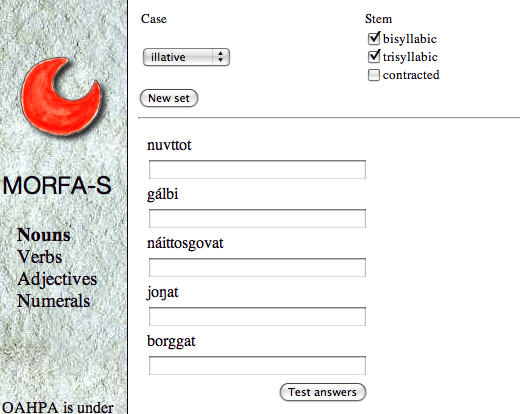
\includegraphics{img/morfaS.png}}\\
\caption{http://victorio.uit.no/oahpa/morfa\_s/}
\label{morfas}
\end{center}
\end{figure}


\subsubsection{Morfa-C}
The student is presented for a set of five questions and a answer with a empty slot and a word in base form. For nouns and adjectives the presentation form can be in singular or plural. After writing the correct word form in the slots, s/he can test the answers. If an answer is incorrect, the student is offered help, which is an explanation about the morphological changes.

After giving in, the student gets a score, and a comment connected to the score. 

The options are for all dialect and book, and in addition one can choose these forms:
\begin{itemize}
\item Nouns: nominative plural and all other cases (with singular and plural mixed). The set contains also some place names to remind the student that also place named are inflected
\item Verbs: indicative present tense, indicative past tense, conditional, potentional, imperative
\item Adjectives: grade: positive comparative and superlative, and as attributive or predicative, all in nominative
\item Numerals: as attribute in different cases mixed, or as head in nominative plural, accusative, illative, locative and comitative (with singular and plural mixed)
\end{itemize}
\vspace{0.5cm}


\begin{figure}[htbp]
\begin{center}
\scalebox{.7}[.7]{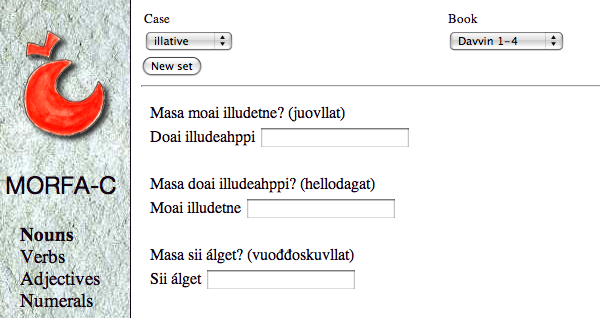
\includegraphics{img/morfaC.png}}\\
\caption{http://victorio.uit.no/oahpa/morfa\_c/}
\label{morfac}
\end{center}
\end{figure}

\vspace{0.5cm}

The sentence generator generates question-answer pairs, and the student writes only one word form into the answer. To get variation, there can be several variables in a pair. The example above generates pairs with numeral used as attribute, and the task in Sámi will be to choose correct case and number for the numeral.\\  


\begin{figure}[htbp]
\begin{center}
\scalebox{.7}[.7]{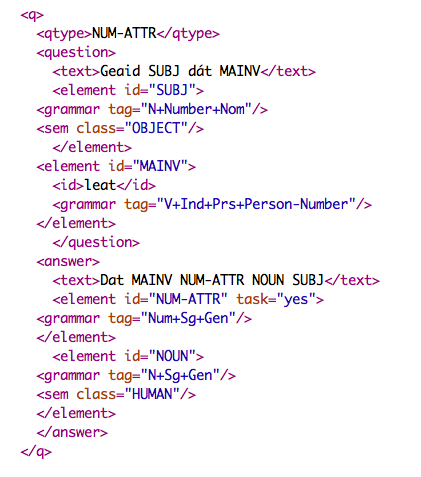
\includegraphics{img/morfa_question.png}}\\
\caption{In Morfa-C the system generates question-answer-pairs. From questions\_numerals.xml.}
\label{questionm}
\end{center}
\end{figure}


We have chosen to use supersets - both HUMAN and OBJECT are quite big supersets. The numeral range is 1-12. This gives many times semantically quite funny sentences. The question-answer pair in Figure \ref{questionm}, can give a text like: \textit{Geaid beavdi dát lea? Dat lea logi vielbeali beavdi.} (Who´s table this is? It is ten cousins’ table.) 

I have discussed it with people, and it seems like that students who are clever in Sámi, like the humour in the sentences. But students on a lower level can get unsure - and they would prefer that the semantic content is realistic all the time.   

In the numeral task we have made variants of the matrices, and marked them with level. In Level 1 the number range is 1-5, and there are only singular numerals because it is easier. Level 2 have both singular and plural numerals. The number range is 1-12, and because of that, there is more humour in the sentences. There are altogether 117 matrice questions, some of them have more than one matrice answer. They are divided into four files, according to POS.




\subsection{Vasta -- open questions}	

In between the "natural" dialogues, mimicking real life dialogues, and the pure grammar training session, inquiring paradigm forms, we have made Vasta - a question-answer drill. The drill has two question types: Yes/no questions and wh-questions. 

There are two motives for making this game type. First, our tailored dialogues in Sahka run the risk of getting quickly consumed. With a QA drill e we may make an indefinite number of questions. Second, the students need to automate the question-answer routine -- inflecting the finite verb correctly and choose the correct case.

The questions are generated, the question and answer are analysed together, and the student gets feedback, like described in \ref{sentencefeedback}. The question matrices are marked with level, so there is a level option. Only one question is presented at a time. The student can answer how s/he likes, but with fill sentence (with finite verb), and with the same verb as in the question. The pronouns are not inclusive.

There are 111 matrice questions divided into levels:
\begin{itemize}
\item Level 1: verb only in present tense, logical cases
\item  Level 2: verb in past tense, and some verbs with oblique cases, use of postpositions, questions in which the student has to answer with case in plural,  numerals and collective numerals in nominative
\item  Level 3: grade: numerals inflected in cases, conditional, time expressions, collective numerals
\end{itemize}
\vspace{0.5cm}


\begin{figure}[htbp]
\begin{center}
\scalebox{.7}[.7]{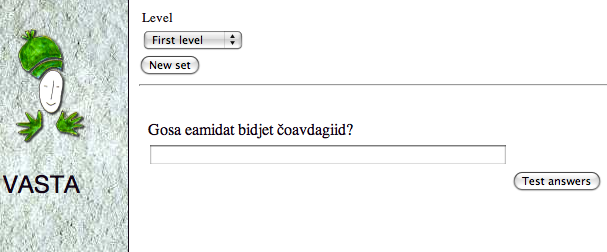
\includegraphics{img/vasta.png}}\\
\caption{http://victorio.uit.no/oahpa/vasta/}
\label{vasta}
\end{center}
\end{figure}

	

\subsection{Sahka -- dialogues}
The idea behind the dialogues is that the student can exercise Sámi in a quite natural way, and at the same time get comments about errors. There will be two kind of feedback: tags for navigation in the dialogue itself, and tags that generate tutorial feedback.

Each dialogue is made to a scenario, and there are underlying pedagogical goals. E.g. in the Grocery-dialogue, the scenario is a shop, and the student is telling what kind of food s/he wants. The underlying pedagogical goal is to exercise inflecting objects in accusative.

In the Get-acquainted-to-dialogues the student can choose an identity for the conversation (s/he chooses a picture). These identities will act as parameters for choice of comments from the computer, and for dialogue topics and dialect forms.

\vspace{0.5cm}
	
Topics:
\begin{itemize}
\item Get acquainted to Hánsa - an adult man living in Kautokeino
\item Get acquainted to Káre - an adult woman living in Karasjok
\item Get acquainted to Lisa - a girl living in Tana
\item Get acquainted to Lemet - a boy living in Tromsø
\item Visit - help to move furniture from one room to another, and have a coffee break
\item Grocery - buying food
\item Comparing in the shop - tell what is cheapest or most expensive, using adjectives in comparative or superlative
\end{itemize}


Each dialogue consists of many branches, and different links according to the student's input. To organize them, we have made different levels:

The dialogue first utterance is a dialogue\_opening and the last utterance is a dialogue\_closing. The student can anytime write that s/he wants to quit, and using the verb \textit{heaitit} will navigate the directly to the dialogue\_closing.

The dialogue consists of topics, and every topic starts with an opening utterance; a comment or a question. In the end of the topic, there is always a closing.  

Every utterance has a name, and one link or alternative links. The alternative links are due to a what kind of tag the question-answer pair gets, e.g. dia-neg or dia-pos, or dia-target to a certain word, e.g. target="hivsset", like in Figure \ref{TV}. There will always be a default, in case there will not be any tag.\\

\begin{figure}[htbp]
\begin{center}
\scalebox{.6}[.6]{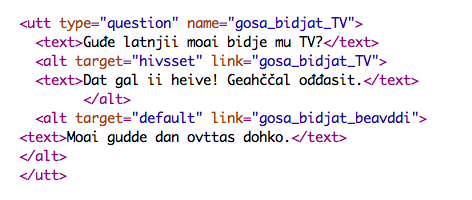
\includegraphics{img/gosabidjatTV.png}}
\caption{The question is "To which room we put the TV?" One of the alternatives for the navigation is due to that the target tag is put to the lemma "hivsset" ( = WC). The comment to the student is "It is not a good idea. Make a new try." From dialogue\_visit.xml.}
\label{TV}
\end{center}
\end{figure}

In Figure \ref{targetIll} we see how the \&dia-target-tag is mapped to the noun in illative.

\begin{figure}[htbp]
\begin{center}
\scalebox{.6}[.6]{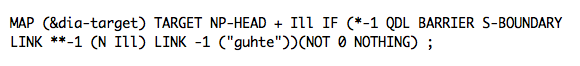
\includegraphics{img/targetIll.png}}
\caption{In the ped-sme.cg3 is a rule for giving target-tag to an noun or pronoun in illative after a question with the interrogate "guhte" + a noun in illative ( = "to which"). This a general rule, not connected to any particular question.}
\label{targetIll}
\end{center}
\end{figure}


A topic is like a module in the dialogue, and it is easy to put an new module after it. The linking makes is possible to make branches. Every utterance have a unique name.  

\subsubsection{Evaluation}
Sahka is a simple dialogue system, and not as advanced as Te Kaitito, which is a bilingual human-machine dialogue system for conversation in English and Maori. The main differences are:

Te Kaitito offers a mixed-initiative dialogue, which means that also the student can ask questions to the program. The program analyses the student's input and can take information to a knowledge base, from which the program computes a response to the user with help of the sentence generator. The system can also make a clarification sub-dialogue, when the user's utterance is ambiguous. \citep{KnotMoorMean200350}

The Te Kaitito research group has introduced a multi-speaker dialogue system in which the system plays several different characters with separate knowledge bases, and who can communicate both with the user and with each other.   
\citep{VlugterKnott06}

The system has an authoring mode, in which the system interacts with a human author setting up the scenario for a single lesson. The author can make assertions and enter questions in order to create an educational agenda for the lesson. The student must demonstrate understanding of each of these during the dialogue in order to move on to the next lesson. \citep{VlugterKnotWeatherall04} \citep{VlugterKnott06}

In Sahka only the program can make initiatives, and all the utterances from the program, are written. We have chosen not to generate utterances. The knowledge base of Sahka is quite limited. The program can store simple information as the student's name, place where s/he lives and his/her car type, for using in as a variable in a tailored utterance. If we want to develop the program with generating of utterances, and a more freely dialogue with mixed initiatives, we should use an analysator, which maps semantic roles to the student's input, despite possible syntactic errors. Giving semantic tags to the lexicon, could be a good help. 

Sahka has no authoring mode; the dialogues have to be written. And the student decides herself when s/he wants to move on to a new dialogue. %Both Sahka and Te Kaitito has in common that the domain is limited. 
 


\subsection{Log}
We have also made a log for the programs. In the log is registered ........ (Saara)

\section{Future plans}
We have planned to change the main lexicon into xml-format, from which we can generate lexicons in lexc-format. The pedagogical lexicon will be integrated in this.

Based on the Internet log and feedback from students, we will improve the feedback systems. We have realized that it is difficult to get teachers and students to try out the programs before they function well. In January 2009 starts a group of students studying bachelor with North Sámi as foreign language at the University of Tromsø, and the OAHPA-programs will be integrated in their instruction. 

We will translate lexicon and grammar into English and Finnish, so these metalanguages will be fully supported. The Finnish metalanguage will make it easier for Sámi students in Helsinki and Oulu to use the programs, and English will be useful for foreign students in Tromsø.

Today we have a quite good analysator for Lule Sámi; but the disambiguator is not fully developed yet. The South Sámi resources should be finished within 2009, and the work for some other sámi languages have been started. The other sámi languages are in an even more threatened situation than North Sámi, with little teaching materials. The programs could be an important supplement. Most sámi languages are talked in several countries with different majority languages, and the infrastructure of these programs is easily adapted to many metalanguages.

But to do this work, we need to work together with teachers to get the content of the programs adapted the student's need.


\newpage

%\begin{spacing}{1}
\par
%\bibliographystyle{jmr} %jmr gives the second author with first name first
\bibliographystyle{jmr}
\bibliography{WAart}
\addcontentsline{toc}{section}{References}
%\end{spacing}

	
\end{document}

	
